\documentclass[tikz]{standalone}

\usepackage{amsmath}
\usepackage{unicode-math}
\usepackage{mathtools}
\usepackage{derivative}

\setmainfont{Stix Two Text}
\setmathfont{Stix Two Math}

\usetikzlibrary{arrows.meta,fit,positioning}

\renewcommand{\familydefault}{\sfdefault}

% prefix equation numbers with section number
\numberwithin{equation}{section}

\DeclarePairedDelimiter{\ceil}{\lceil}{\rceil}
\DeclarePairedDelimiter{\floor}{\lfloor}{\rfloor}
\DeclarePairedDelimiter{\abs}{\lvert}{\rvert}
\DeclarePairedDelimiter{\norm}{\lVert}{\rVert}
\DeclarePairedDelimiter{\bra}{\langle}{\rvert}
\DeclarePairedDelimiter{\ket}{\lvert}{\rangle}
\DeclarePairedDelimiter{\expval}{\langle}{\rangle}
\DeclarePairedDelimiter{\norder}{\mathcolon}{\mathcolon}
\DeclarePairedDelimiter{\anorder}{\typecolon}{\typecolon}
	
\newcommand{\laplace}{\mbfnabla^2}
\newcommand{\trans}{{\scriptscriptstyle\mathsf{T}}}

\newcommand{\vdot}{\cdot}
\newcommand{\vcross}{\vectimes}
\newcommand{\vb}[1]{\symbfup{#1}}
\newcommand{\vu}[1]{\hat{\vb{#1}}}
\newcommand*\dd[2][\relax]{\mathop{\ifx\relax#1\odif{#2}\else \odif[order={#1}]{#2}\fi\,}}

\newcommand{\vacuum}{\ket*{\vb{0}}}

\DeclareMathOperator{\trace}{Tr}
\DeclareMathOperator{\sinc}{sinc}

\AtBeginDocument{
	\let\Re\relax
	\let\Im\relax
	\DeclareMathOperator{\Re}{Re}
	\DeclareMathOperator{\Im}{Im}

	\renewcommand{\div}{\mathop{\mbfnabla\vdot}}
	\newcommand{\curl}{\mathop{\mbfnabla\vectimes}}
}

\DeclarePairedDelimiterX{\comm}[2]{[}{]}{#1,#2}

\DeclarePairedDelimiterX{\braket}[2]{\langle}{\rangle}{#1\delimsize\vert#2}
\DeclarePairedDelimiterX{\ketbra}[1]{\lvert}{\rvert}{#1\rangle\delimsize\langle#1}



\begin{document}
	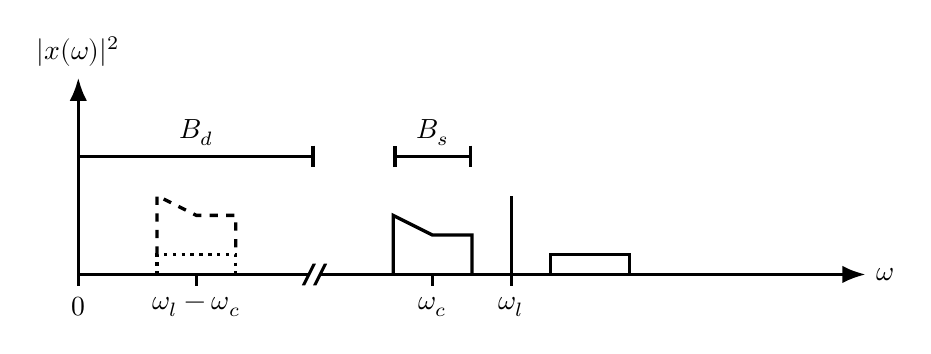
\begin{tikzpicture}
		\draw[very thick, -Latex] (0,0) -- ++(0,2.5) node[above] {$\abs{x(\omega)}^2$};
		\draw[very thick, {-Bar[slant=.5]}] (0,0) -- (2.95,0);
		\draw[very thick, {Bar[slant=.5]-Latex}] (3.05,0) -- (10,0) node[right] {$\omega$};

		\draw[very thick] (0,0) -- ++(0,-0.15) node[below] {$0$};
		\draw[very thick] (1.5,0) -- ++(0,-0.15) node[below] {$\omega_l-\omega_c$};
		\draw[very thick] (4.5,0) -- ++(0,-0.15) node[below] {$\omega_c$};
%		\draw[very thick] (6.5,0) -- ++(0,-0.15) node[below] {$\omega_i$};
		\draw[very thick] (5.5,0) -- ++(0,-0.15) node[below] {$\omega_l$};

		\draw[very thick, dotted] (1,0) -- ++(0,0.25) -- ++(1,0) -- ++(0,-0.25);	
		\draw[very thick, dashed] (1,0.25) -- ++(0,0.75) -- ++(0.5,-0.25) -- ++(0.5,0) -- ++(0,-0.5);
		\draw[very thick] (4,0) -- ++(0,0.75) -- ++(0.5,-0.25) -- ++(0.5,0) -- ++(0,-0.5);
		\draw[very thick] (5.5,0) -- ++(0,1);
		\draw[very thick] (6,0) -- ++(0,0.25) -- ++(1,0) -- ++(0,-0.25);
		
		\draw[Bar-Bar, very thick] (4,1.5) -- ++(1,0) node[midway, above] {$B_s$};
		\draw[-Bar, very thick] (0,1.5) -- ++(3,0) node[midway, above] {$B_d$};
	\end{tikzpicture}
\end{document}
